\documentclass[11pt,a4paper]{article}
\usepackage[margin=2.2cm]{geometry}
\usepackage{graphicx,amsmath,amssymb,booktabs,xcolor,hyperref,float,caption}
\captionsetup{font=small,labelfont=bf}
\graphicspath{{figs/}}
\DeclareGraphicsExtensions{.pdf,.png}
\newcommand{\half}{\tfrac12}
\newcommand{\la}{\ell_a}
\newcommand{\kT}{k_BT}
\newcommand{\verdict}[2]{\textbf{\textcolor{#1}{[#2]}}}
\title{Crowded wall layers tilt less\\[2pt]\large What we measured, what we tested, and what is still open}
\author{Notes for B.~Loewe and T.~N.~Shendruk (prepared with Claude)}
\date{16 October 2026}
\begin{document}
\maketitle

\begin{abstract}
The wall $+\half$ defects of an overcharged active cavity tilt from the wall normal. At leading order the tilt follows the flow-alignment law $\tau=\arccos(1/\lambda)$, $60^\circ$ at $\lambda=2$. With 10 seeds we find that this holds only for sparse wall layers. The tilt falls steadily as the wall defects crowd together, from $\approx64^\circ$ at spacings above 20 cells to $\approx42^\circ$ at 7 cells. The fall collapses on the wall-defect spacing. It appears in circles, ellipses and Cassini ovals, and it also appears in passive layers driven by an imposed vortex. We tested the candidate explanations in turn:
\begin{itemize}
\item measurement artefacts;
\item a weaker mean wall shear;
\item the defects' own active flow;
\item the finite-shear correction to the tilt law;
\item static elasticity, at a flat wall and in the circle;
\item the bulk spiral;
\item the continuum Q-tensor model in flat and circular geometries.
\end{itemize}
Each test either fails or explains only part of the drop. One combination does order all the data: core depth times the square root of the wall shear rate, $d\sqrt{s}$, i.e.\ depth over the alignment length. The continuum models never produce tilts below $\arccos(1/\lambda)$. The physics behind the drop below $60^\circ$ is therefore still open, and it appears to be specific to the MPCD wall layer. The last section lists what the paper can safely claim and what to test next.
\end{abstract}

\section{Background and definitions}

\paragraph{Tilt law.} Relative to the wall normal, the anchored director turns by $(k-1)\phi$. A wall $+\half$ at azimuth $\phi_j$ therefore has its tilt locked to its position:
\begin{equation}
\tau_j=(2k-2)\phi_j+c .\label{eq:lock}
\end{equation}
A common tilt of the layer is a rigid shift of its registry. In shear next to a no-slip wall the far-field director settles at the Leslie angle $\theta_L$, with $\cos2\theta_L=1/\lambda$. The layer slides along this zero mode until the far field is aligned, so $\tau=2\theta_L=\arccos(1/\lambda)$. The master document adds a finite-shear correction from the torque passed through the band between wall and core:
\begin{equation}
\tau=\arccos\frac1\lambda+d\sqrt{\frac{\gamma_1 s}{K}}\,(\lambda^2-1)^{-1/4},\label{eq:corr}
\end{equation}
where $d$ is the core depth and $s$ the wall shear rate. The correction is always positive.

\paragraph{Definitions used throughout.}
\begin{itemize}
\item \textbf{Tilt.} $\tau=\psi-\theta_n$, the angle between the radial arm of the $+\half$ comet (the defect angle $\psi$ in \texttt{defects.dat}) and the outward wall normal. We checked analytically that the MPCD defect angle, the flat-wall direction of $\nabla\!\cdot\!Q$ and the ``head'' of the analytic calculations are all this same direction.
\item \textbf{Coherence.} $C=|\langle e^{i\tau_j}\rangle|$ over the wall defects of one frame (wall = within 4 cells of the wall).
\item \textbf{Tilt of the coherent layer.} The median over frames with $C>0.9$ of $|\arg\langle e^{i\tau_j}\rangle|$.
\item \textbf{Spacing.} $a=2\pi R/(2k-2)$ in circles, and the local site spacing $a(s)=\pi/(2\pi k/P-\kappa(s))$ in elongated cavities.
\item \textbf{Wall density.} $\rho=k/\pi R$.
\item \textbf{Alignment length.} $\ell_E=\sqrt{K/(\gamma_1 s\sqrt{\lambda^2-1})}$, the thickness of the shear boundary layer over which the director turns from the anchoring to $\theta_L$.
\end{itemize}

\section{The observation}

\begin{figure}[H]\centering
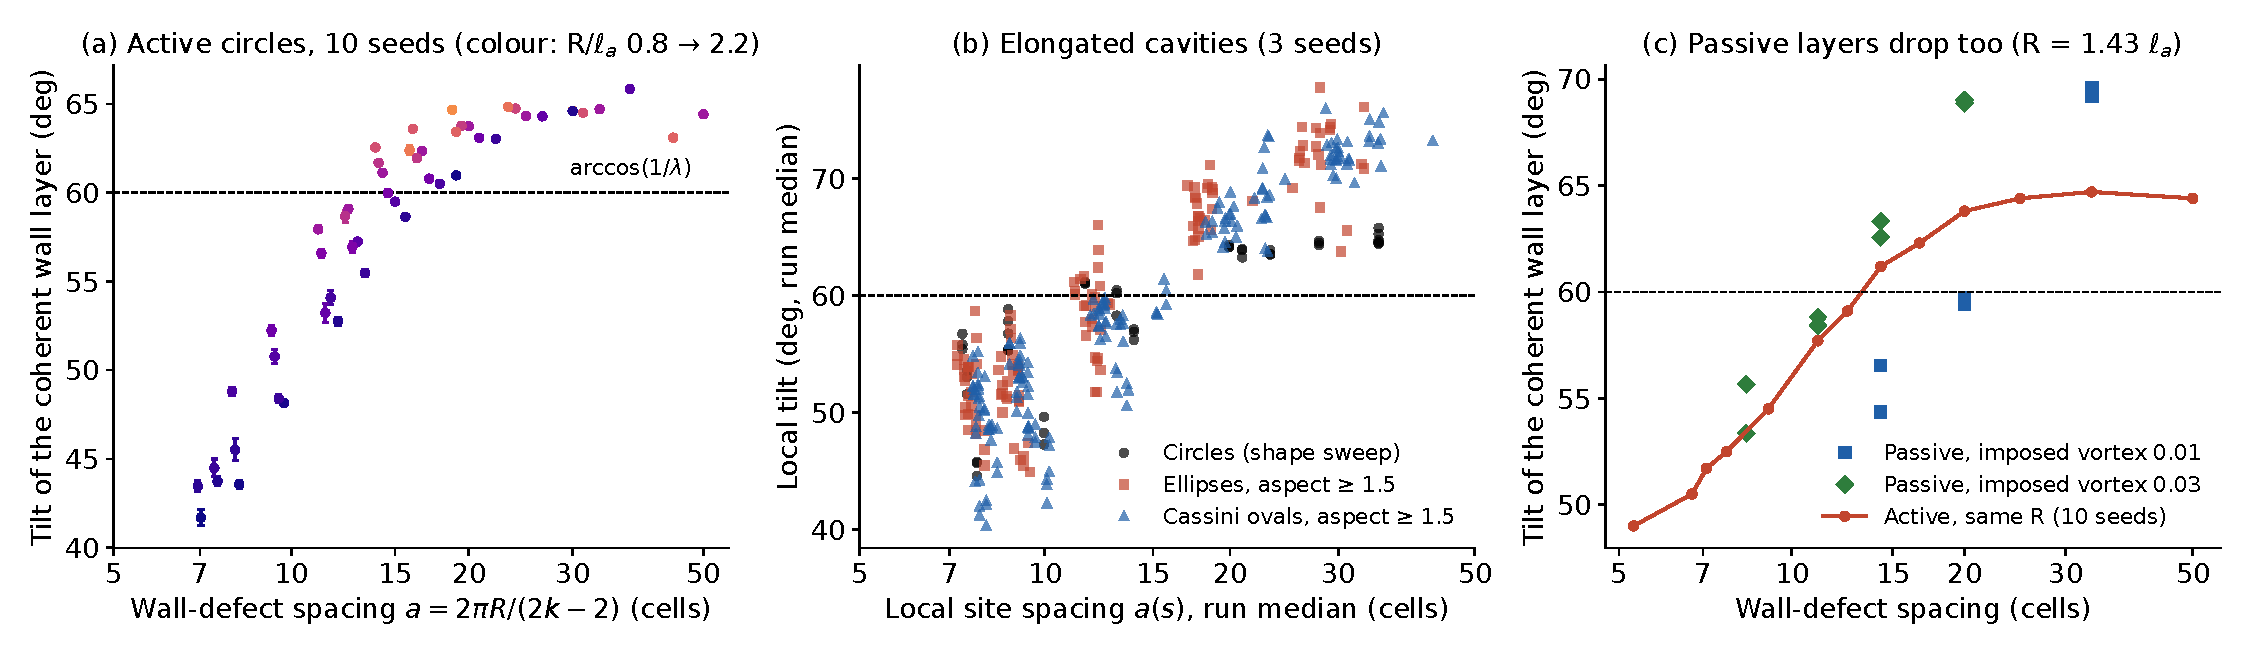
\includegraphics[width=\textwidth]{fig1_observation}
\caption{(a) Tilt of the coherent wall layer in active MPCD circles: $\lambda=2$, $\zeta=0.07$, $k=2$--10, $0.8\le R/\la\le2.2$, 10 seeds (mean $\pm$ s.e.\ per $(k,R)$). (b) Elongated cavities: local tilt of locally coherent triplets of wall defects against the local site spacing (run medians, 3 seeds). (c) Passive layers under an imposed vortex (two amplitudes) and active layers at the same radius $R=1.43\,\la$.}\label{fig:obs}
\end{figure}

\begin{itemize}
\item \textbf{The drop.} The tilt falls from $64.6^\circ$ ($\rho\approx0.04$) through 63.0, 59.2, 54.7 and 49.4 to $44.2^\circ$ ($\rho\approx0.14$). These are 506 runs with 10 seeds each (Fig.~\ref{fig:obs}a).
\item \textbf{Collapse on spacing.} A quadratic fit in $\log a$ leaves $1.7^\circ$ rms, against a raw spread of $7.0^\circ$. Fits in $k$ or $R$ alone leave $5$--$6^\circ$ (Fig.~\ref{fig:heat}). The tilt sits at $\approx64^\circ$ for $a\gtrsim20$ cells, crosses $60^\circ$ at $a\approx15$ and reaches $\approx42^\circ$ at $a=7$. A phenomenological form $\tau=\tau_L/(1+(a^*/a)^2)$ fits with $\tau_L=67.4^\circ$, $a^*=5.35$ cells and $2.0^\circ$ rms; it is a description, not a derivation.
\item \textbf{Elongated cavities} (Fig.~\ref{fig:obs}b). Measured from the local normal (the lock holds there too: resultant 0.94--0.98), ellipses and ovals show the same fall. Their sparse layers tilt more than circles, at $66$--$71^\circ$.
\item \textbf{Passive layers} (Fig.~\ref{fig:obs}c). Under an imposed vortex the tilt falls just as steeply, $69^\circ\to54^\circ$ between $a=20$ and $7.7$ at swirl 0.03. A stronger swirl raises the tilt at fixed spacing ($k=6$: $59.5^\circ$ at 0.01, $69^\circ$ at 0.03). Activity is therefore not required for the drop.
\end{itemize}

\begin{figure}[H]\centering
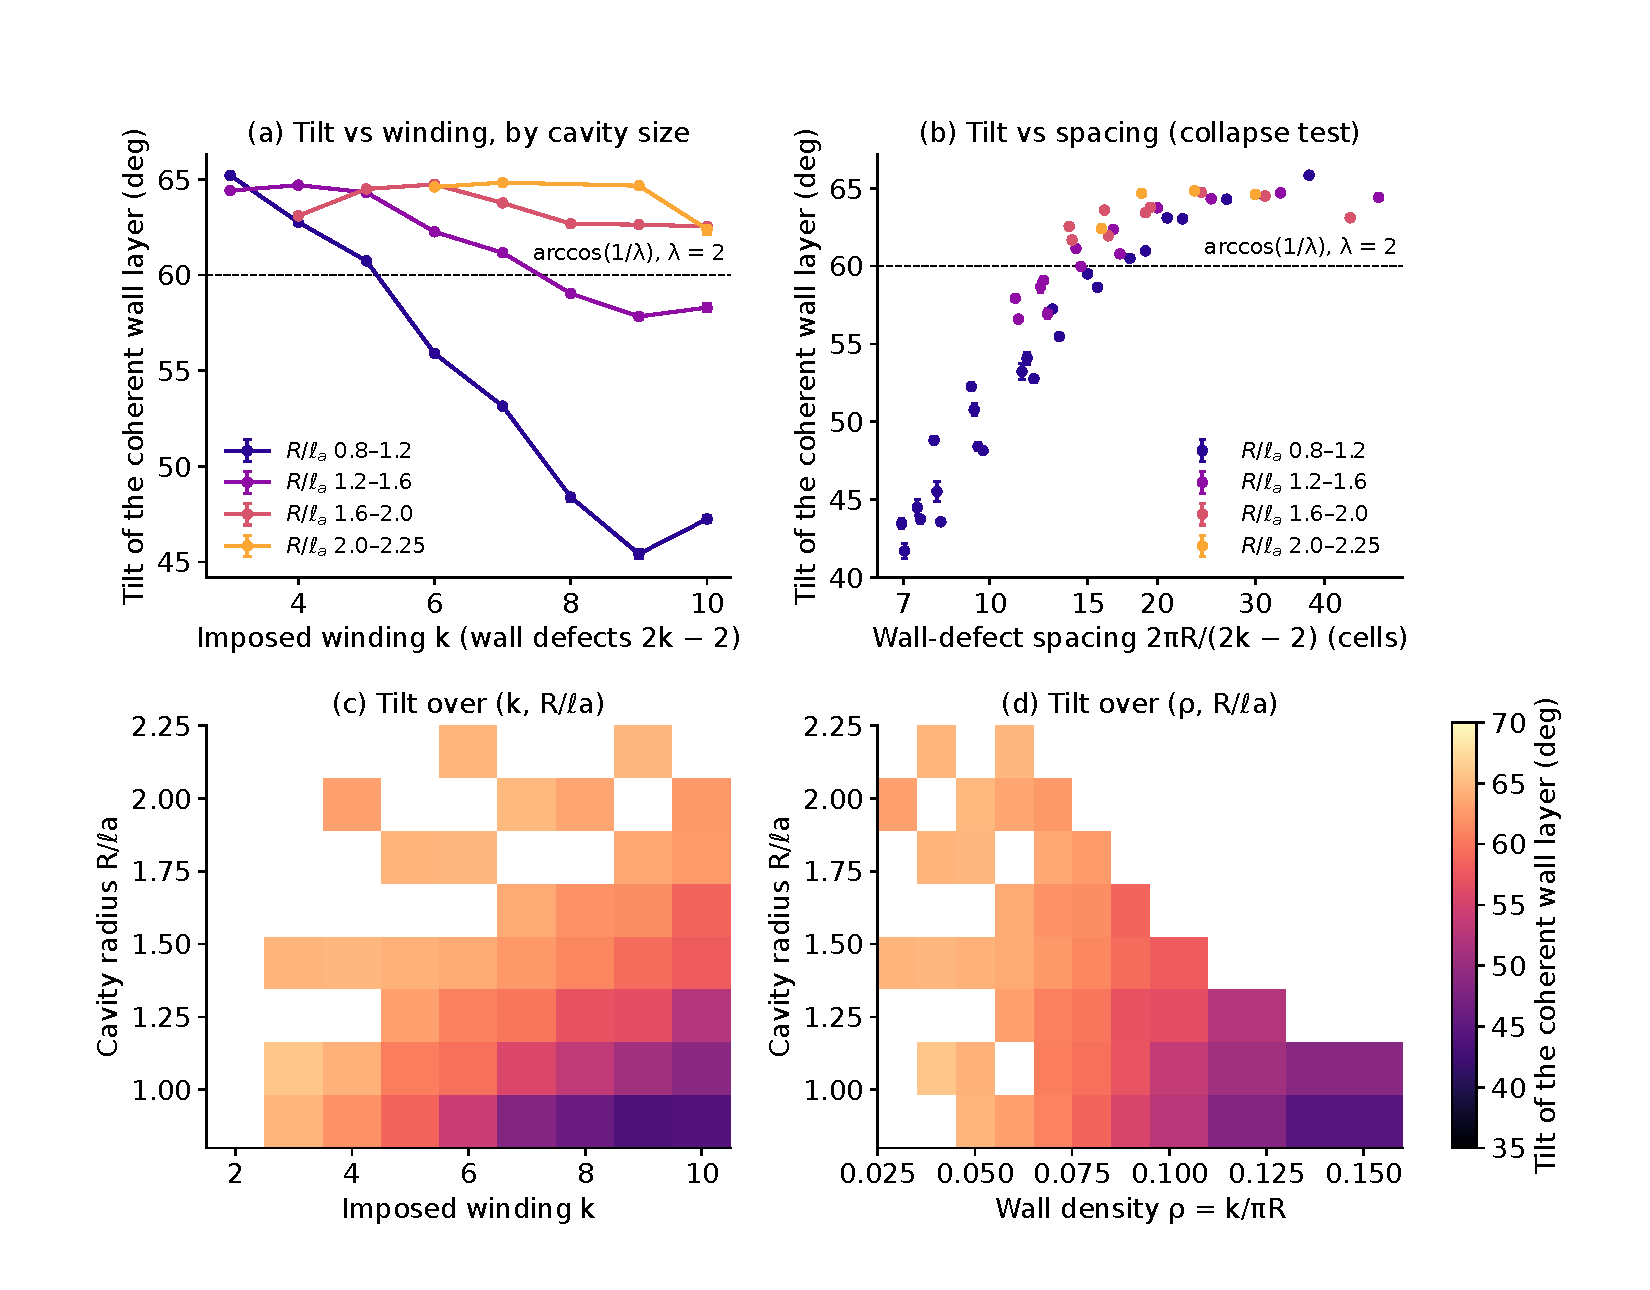
\includegraphics[width=0.85\textwidth]{fig_tilt_k}
\caption{Active circles (10 seeds). (a) Tilt against $k$ for four size bands. (b) Tilt against spacing: the collapse. (c, d) Tilt over $(k,R/\la)$ and over $(\rho,R/\la)$.}\label{fig:heat}
\end{figure}

\section{Test 1: is it a measurement effect? \verdict{red}{Mostly no}}

\begin{figure}[H]\centering
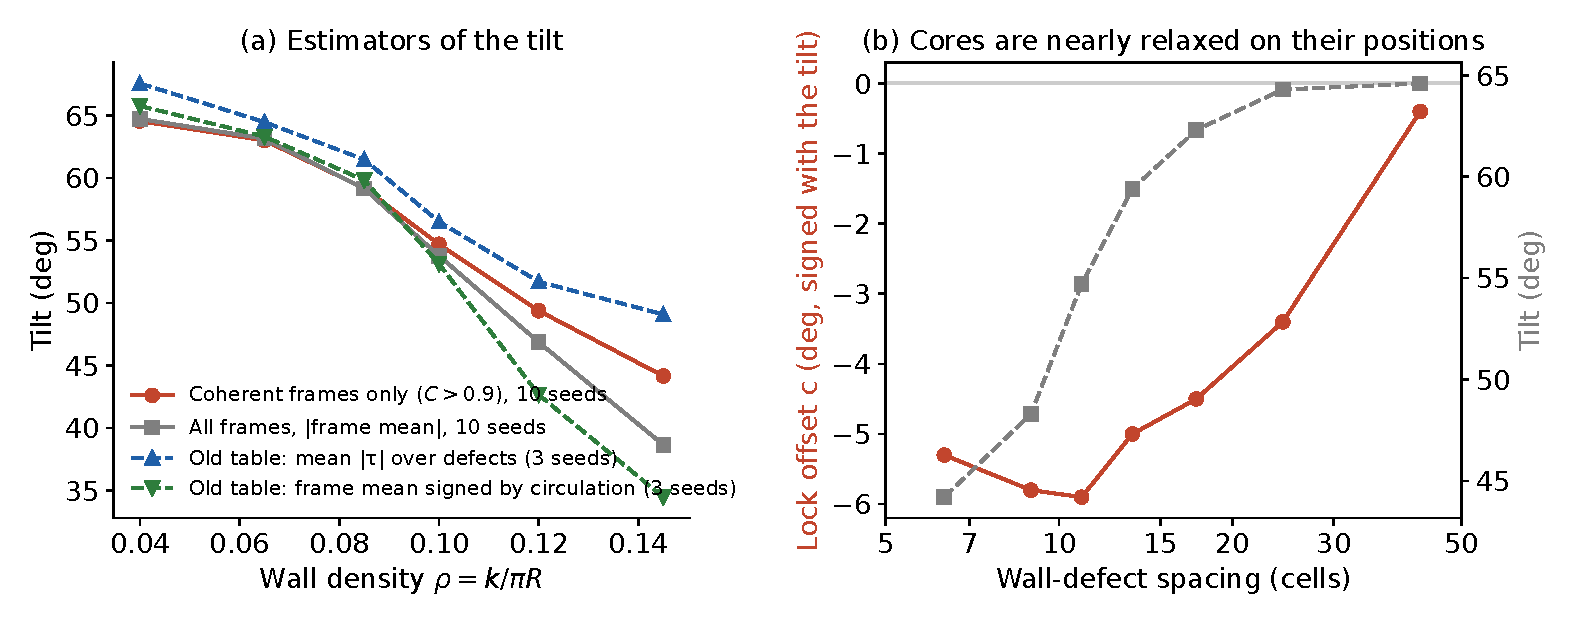
\includegraphics[width=0.85\textwidth]{fig2_measurement}
\caption{(a) Estimators of the tilt against wall density. The earlier table value signed by the circulation (3 seeds) overstates the drop at high $\rho$; the coherent-frame tilt does not. (b) Orientation offset $c$ of the cores from the lock, signed with the tilt, and the tilt itself, against spacing.}\label{fig:meas}
\end{figure}

\paragraph{Estimators.} The first report of the drop ($33$--$43^\circ$ at $\rho\ge0.12$) used the frame-mean tilt signed by the circulation and sampled every 100 t.u. Crowded layers scatter more and switch circulation more often, which pulls that average down. In addition, the column named \texttt{tilt\_coh} in that table is the magnitude of the mean angle, not the coherence. Restricting to frames in which the layer clearly shares one tilt ($C>0.9$) removes both effects. The drop survives, at a smaller size: $44^\circ$ instead of $38^\circ$ at $\rho\approx0.14$ (Fig.~\ref{fig:meas}a).

\paragraph{Are the cores relaxed?} Your point was that the logarithmic interaction assumes each defect's orientation has relaxed to its minimum. Unrelaxed orientations exert torques. We measured the offset $c$ of each frame's cores from the lock, Eq.~\eqref{eq:lock}. Sparse layers are relaxed ($c=-0.4^\circ$). Crowded layers are twisted back toward the normal by $5$--$6^\circ$, and the resultant falls from 0.99 to 0.97 (Fig.~\ref{fig:meas}b). This is real, but it accounts for only $\approx5^\circ$ of the $\approx20^\circ$ drop. The rest is the registry: crowded defects sit closer to their homeotropic sites.

\section{Test 2: is it the flow? \verdict{orange}{Partly}}

\begin{figure}[H]\centering
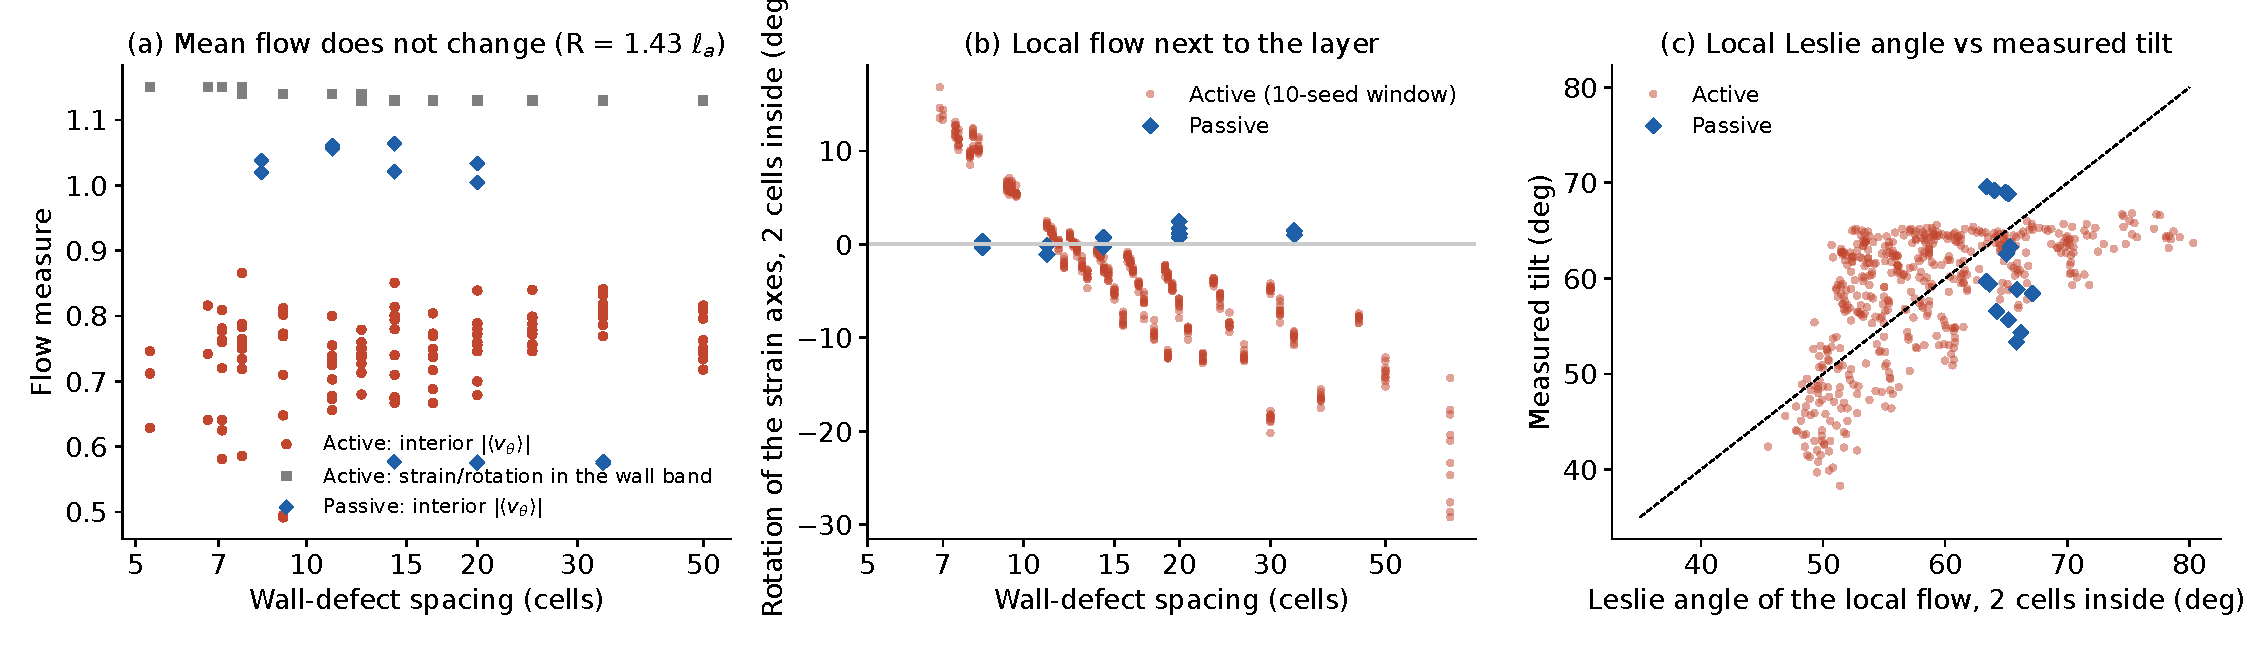
\includegraphics[width=\textwidth]{fig3_flow}
\caption{(a) Interior circulation and strain/rotation ratio in the wall band at fixed $R=1.43\,\la$: neither changes with spacing. (b) Rotation of the principal strain axes two cells inside the layer, in each wall defect's own frame: active layers (10-seed window) and passive layers. (c) Leslie angle of that local flow against the measured tilt.}\label{fig:flow}
\end{figure}

\paragraph{Mean wall shear: \verdict{red}{fails}.} Your first idea was that the layer's self-flow opposes the circulation, so a denser layer weakens the wall shear. At fixed $R$, however, the azimuthally averaged wall-band shear is the same for every $k$ (strain $\approx0.09$--$0.10$, strain/rotation 1.10--1.15), and so is the interior circulation. The tilt law also predicts no dependence on the shear magnitude, only on the strain/rotation ratio, and that ratio is unchanged.

\paragraph{Local flow at the layer: \verdict{orange}{works for active, fails for passive}.} The defects' flow lobes repeat with period $a$ and cancel in the azimuthal mean, so we sampled the flow in each wall defect's frame.
\begin{itemize}
\item \textbf{Active layers.} Two cells inside the layer the strain axes rotate steadily, from $-17^\circ$ (sparse) through 0 at $a\approx13$ to $+11^\circ$ (crowded). The Leslie angle of that local flow tracks the measured tilt bin by bin: $49.6/52.0/57.0/65.1^\circ$ against $45.8/51.2/60.8/64.4^\circ$ for $a$ = 5--8/8--12/12--20/20--60 (Fig.~\ref{fig:flow}b,c).
\item \textbf{Passive layers.} The local flow is plain wall shear at every spacing: strain-axis rotation $0\pm1^\circ$, local Leslie angle $63$--$67^\circ$. The tilt still falls.
\item \textbf{The active core.} It carries the defect's own extensional self-flow: $e_{xx}\approx-0.02$, strain axes rotated by $-21$ to $-27^\circ$ at the core. Along the wall this flow runs against the circulation in sparse layers.
\end{itemize}
\emph{Reading:} the local-flow change in active layers is the active self-flow and goes with the tilt. It is not needed for the drop, because passive layers fall equally with an unchanged local flow. In active layers it is most likely a consequence of the crowded, less tilted layer rather than its cause.

\section{Test 3: is it elastic? \verdict{red}{Not as a static effect}}

\begin{figure}[H]\centering
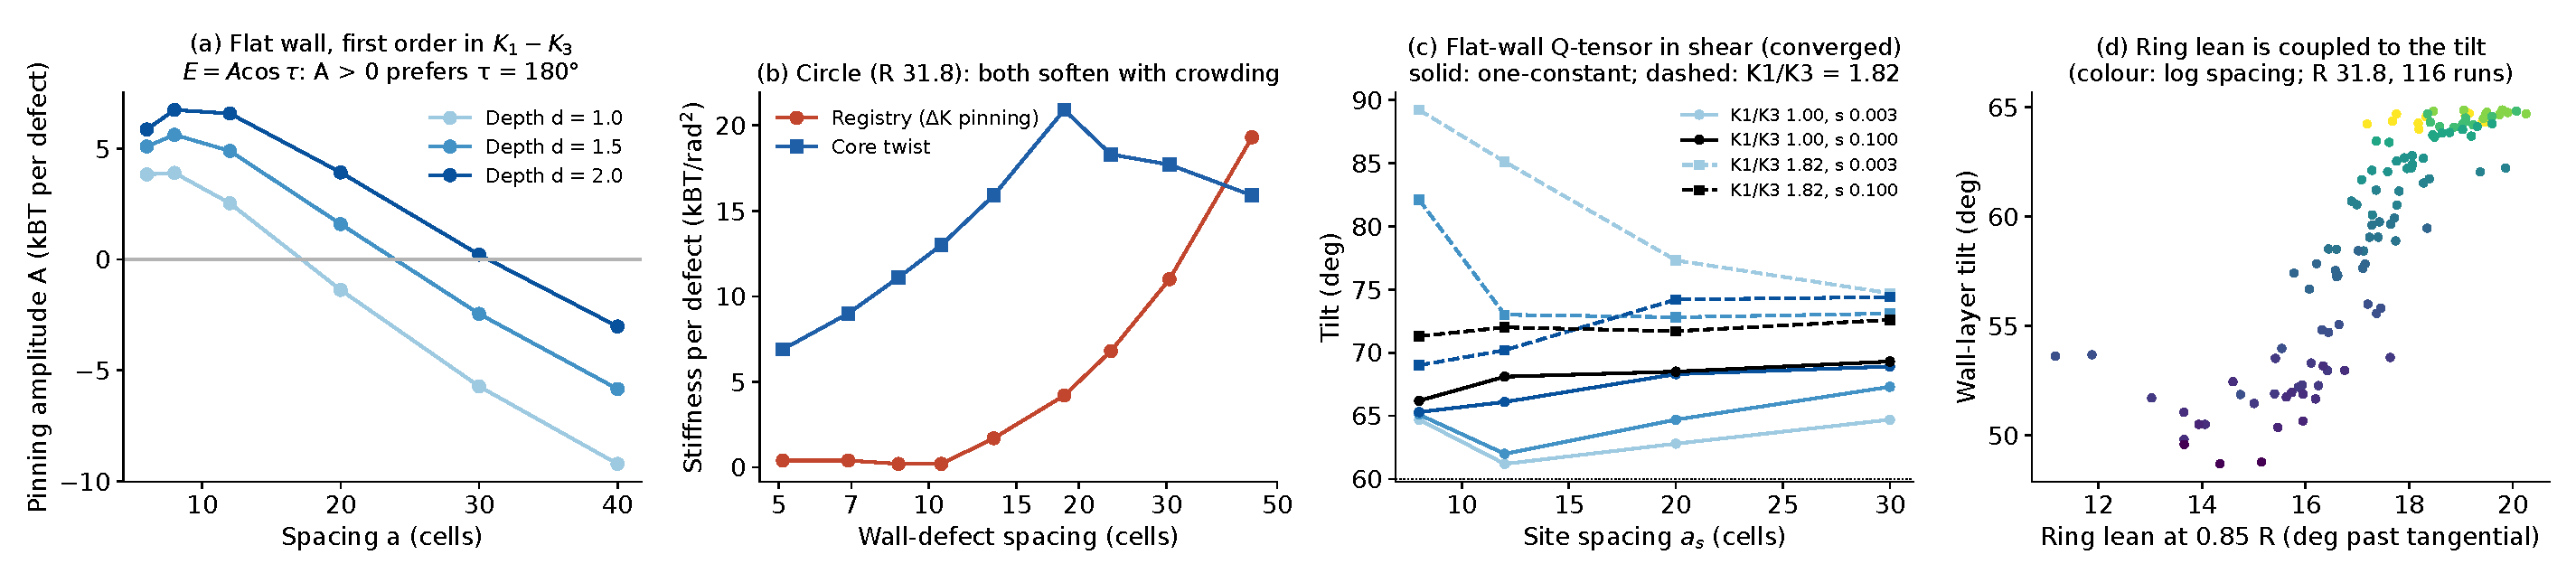
\includegraphics[width=\textwidth]{fig4_elastic}
\caption{(a) Flat-wall registry pinning at first order in $K_1-K_3$ (exact one-constant field plus perturbation): $E(\tau)=A\cos\tau$ per defect, with $A>0$ preferring $\tau=180^\circ$. (b) Circle ($R=31.8$, $2k-2$ ring plus central $+1$): registry stiffness from $\Delta K$ pinning and core-twist stiffness at fixed positions, per defect. (c) Flat-wall Landau--de Gennes model in simple shear (converged): tilt against site spacing for one-constant (solid) and $K_1/K_3=1.82$ (dashed) at several shear rates. (d) Lean of the ordered director ring at $0.85R$ against the wall tilt (116 runs at $R=31.8$).}\label{fig:el}
\end{figure}

\paragraph{Why elasticity was a natural suspect.} The spacing sets the drop, and spacing is an elastic length. With equal splay and bend constants the registry shift (the tilt) is an exact zero mode, so only the flow can set it. With $K_1\ne K_3$ the zero mode is broken, and the elastic energy prefers some untilted state. The idea was that crowding makes this elastic preference win over the flow.

\paragraph{What the calculations give.}
\begin{itemize}
\item \textbf{Circle, analytic, first order in $\Delta K=9.45\,\kT$.} The minimum is at $\tau=0$ (radial arm at the wall), with a barrier of 80--110\,$\kT$ at $k=6$. The registry stiffness, however, collapses with crowding: 19 (k\,3) $\to$ 4 (k\,6) $\to$ 0.2--0.4\,$\kT$/rad$^2$ ($k\ge10$). The core-twist stiffness (your unrelaxed-orientation channel) also softens, from 16--21 to 7\,$\kT$/rad$^2$. Both channels make crowded layers \emph{easier} to tilt, not harder (Fig.~\ref{fig:el}b). The large circle barrier is a bulk effect: a registry shift rotates the whole central $+1$ between aster and vortex, and $K_1>K_3$ favours the vortex.
\item \textbf{Flat wall, analytic, first order.} With that bulk term absent, $E=A\cos\tau$ with $A$ of a few $\kT$ per defect. Crowded or deeper layers prefer $\tau=180^\circ$ and sparse or shallow ones prefer $0^\circ$; the sign changes at $a\approx15$--30 (Fig.~\ref{fig:el}a). This local term pushes crowded layers toward \emph{more} tilt.
\item \textbf{Flat wall, Landau--de Gennes with $K_1/K_3=1.82$.} At rest the layer converges to $\tau=180^\circ$, the same as the analytic flat wall. (Earlier ``rest tilts'' of 51--152$^\circ$ were unconverged.) Under shear the tilt is 69--89$^\circ$ and \emph{higher} at small spacing. With one constant it is 61--69$^\circ$ and rises mildly with spacing. It never falls below $60^\circ$ (Fig.~\ref{fig:el}c).
\end{itemize}

\paragraph{The bulk spiral.} Behind a tilted layer the bulk sees a spiral boundary condition. In MPCD there is no centred $+1$: the interior is disordered (orientational order $\le0.2$ for $r<0.6R$). There is an ordered, nearly tangential ring next to the layer (order 0.7 at 5 cells inside). Its lean past tangential follows the tilt in sign and trend, at about half the amplitude: $18.5$--$19.5^\circ$ for sparse and $14.4$--$15.7^\circ$ for crowded layers at $0.85R$. It is tightly coupled to the tilt seed by seed (correlation $+0.70$ within $k$; Fig.~\ref{fig:el}d). It does not, however, explain the drop beyond spacing: the residual goes from $0.86^\circ$ to $0.71^\circ$. Its effect on the circulation is also small: the interior flow falls only 5--8\%.

\emph{Reading:} static elasticity at the wall has the wrong sign to explain the drop. The bulk-spiral (vortex) preference acts in the right direction, but in MPCD it is carried only by the ring next to the layer, and its strength there is not known.

\section{Test 4: depth and the alignment length \verdict{orange}{Orders the data, mechanism open}}

\begin{figure}[H]\centering
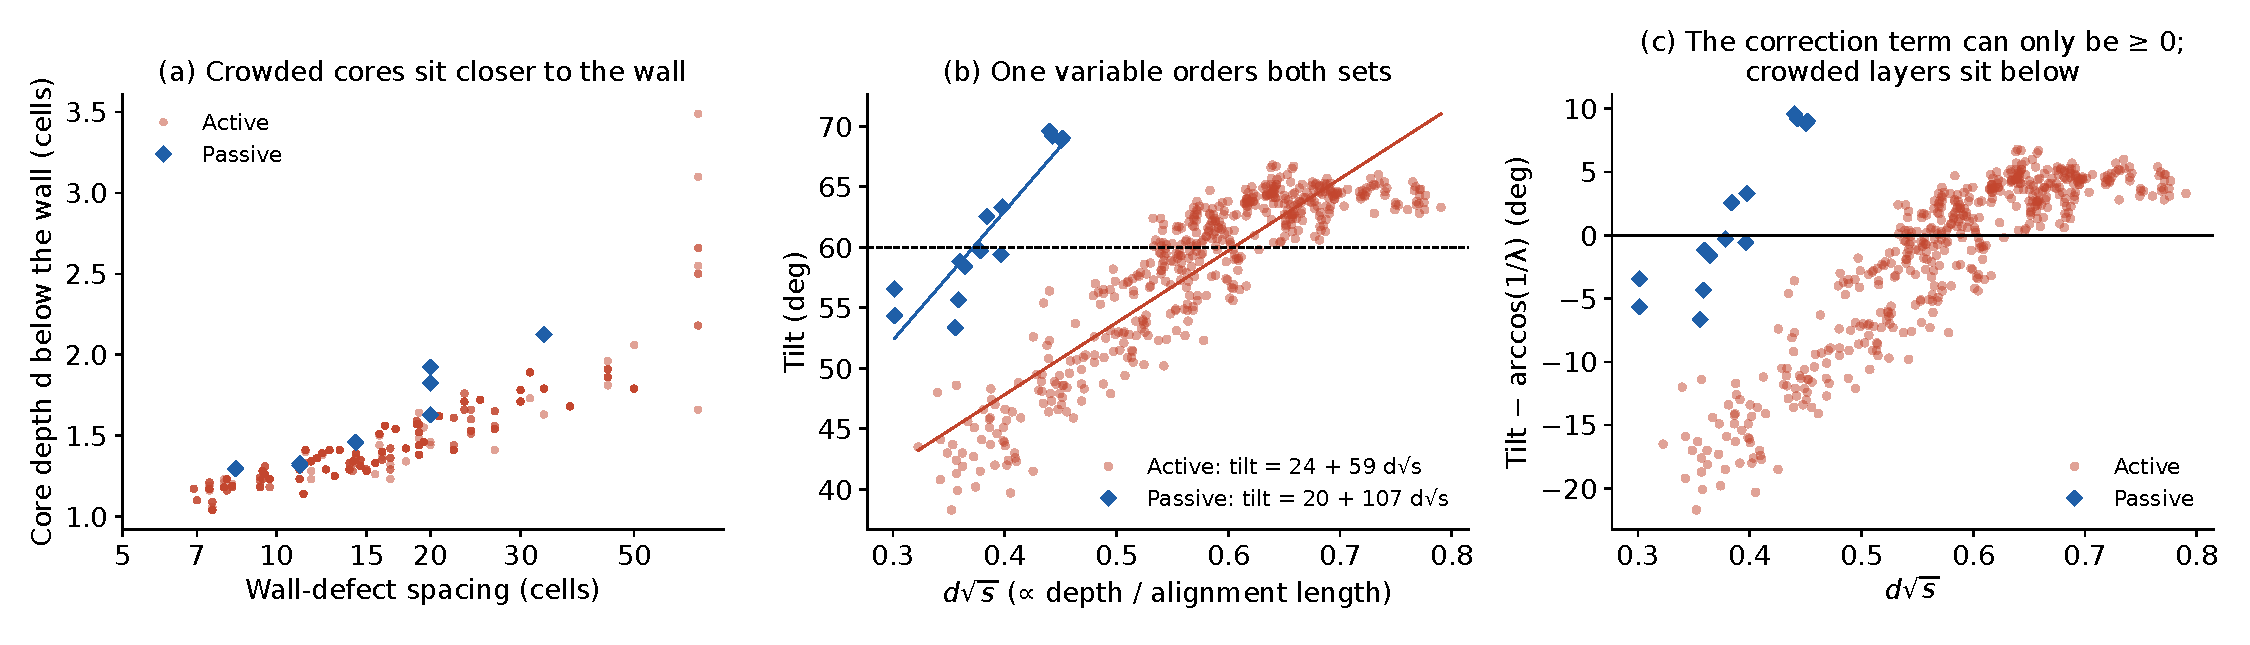
\includegraphics[width=\textwidth]{fig5_depth}
\caption{(a) Core depth below the wall against spacing, active and passive. (b) Tilt against $d\sqrt{s}$ with linear fits. (c) Tilt minus $\arccos(1/\lambda)$: the correction term of Eq.~\eqref{eq:corr} can only be positive.}\label{fig:depth}
\end{figure}

\paragraph{What fits.} Crowded cores sit closer to the wall: depth $\approx1.8\to1.3$ cells (active) and $2.1\to1.3$ (passive) between sparse and crowded layers. The tilt is linear in $d\sqrt{s}$ for both sets:
\begin{itemize}
\item passive: $\tau\approx20^\circ+107\,d\sqrt{s}$, with $2.3^\circ$ rms (raw $5.6^\circ$);
\item active: $\tau\approx24^\circ+59\,d\sqrt{s}$, with $2.9^\circ$ rms (raw $6.8^\circ$).
\end{itemize}
Both fits beat spacing alone ($3.4^\circ$/$3.5^\circ$) and depth alone ($4.2^\circ$/$4.3^\circ$). The shear rate matters at fixed depth: passive $k=8$ at $d=1.46$ gives $55.5^\circ$ at $s=0.043$ and $63^\circ$ at $s=0.072$. Since $d\sqrt{s}\propto d/\ell_E$, the variable that orders the data is the core depth measured in units of the shear boundary layer.

\paragraph{Why the correction term itself fails.} Eq.~\eqref{eq:corr} has the right trend on the sparse side: as $d$ shrinks the positive excess shrinks, which explains a fall from 64--69$^\circ$ toward $60^\circ$. But the term is positive by construction, so it cannot produce tilts below $60^\circ$, and crowded layers sit at 44--55$^\circ$ (Fig.~\ref{fig:depth}c). Fitted with its leading term fixed at $60^\circ$, it leaves residuals that still correlate with spacing ($+0.8$). The fitted intercepts of 20--24$^\circ$ say that, in the data, the tilt is not ``$60^\circ$ plus a correction'' at all.

\paragraph{A hypothesis that would explain the sign.} The layer's periodic distortion extends only $\sim a/2\pi$ from the wall, and the alignment length in MPCD is $\ell_E\approx1.4$--$2.7$ cells. For sparse layers ($a/2\pi\approx3$--8) the distortion reaches past $\ell_E$, and the layer locks to a fully aligned far field. For crowded layers ($a/2\pi\approx1$--1.6) it lies inside the boundary layer, so the layer would lock to a field that has only partly rotated toward $\theta_L$. This would give $\tau<60^\circ$. It needs something that resists the zero-mode sliding, because the one-constant continuum shows no drop even when $a/2\pi\ll\ell_E$.

\paragraph{Continuum test of this regime: \verdict{red}{inconclusive}.} In the flat-wall Q-tensor model $d/\ell_E$ stays at 0.05--0.29, while MPCD has 0.5--1.2. At strong shear ($s=0.3$) the continuum defect is pushed onto the first grid row, and at $s=1$ it is absorbed into the wall. The continuum cannot reach the MPCD regime, where the cores stay 1.2--2 cells deep.

\section{Test 5: the continuum in a circular cavity}

\paragraph{Passive disk with the measured no-slip vortex imposed.} $R=31.8$, $\lambda=2$, $k=4$--20 (spacing 31 down to 4.8 cells), with the $2k-2$ ring seeded. At $U=1$ the layer is coherent at every $k$. The tilt falls only mildly toward $\arccos(1/\lambda)$, never below it:
\begin{itemize}
\item one constant: 67.9 (spacing 31) $\to$ 66.7 $\to$ 64.7 $\to$ 64.8 $\to$ 63.8 $\to$ 64.2 $\to$ $62.3^\circ$ (spacing 4.8);
\item $K_1/K_3=1.82$ with the MPCD Jeffery law: 67.4 $\to$ 65.9 $\to$ 64.8 $\to$ 65.0 $\to$ 64.0 $\to$ 64.9 $\to$ $62.3^\circ$.
\end{itemize}
At $U=0.3$ the crowded rings often fail to eject (coherence 0.6--0.8). The same geometry in MPCD gives $69\to54^\circ$. A mild fall toward $60^\circ$ is what the correction term predicts; the drop below $60^\circ$ is absent.

%%ACTIVE%%

\section{Summary: what works, what fails}

\begin{center}\small
\begin{tabular}{p{4.1cm}p{1.9cm}p{8.6cm}}
\toprule
Candidate & Verdict & Why \\
\midrule
Measurement / averaging & part & Inflated the drop ($38^\circ$ vs $44^\circ$ at $\rho\approx0.14$); a real drop survives in coherent frames. \\
Unrelaxed core orientation & part & Real ($c\approx-5^\circ$ when crowded), but only $\approx5^\circ$ of $\approx20^\circ$. \\
Weaker mean wall shear & fails & Mean band shear and circulation independent of $k$ at fixed $R$. \\
Active self-flow at the layer & fails as cause & Tracks the tilt in active layers; passive layers drop without it. \\
Correction term, Eq.~\eqref{eq:corr} & part & Explains the fall from 64--69$^\circ$ to 60$^\circ$; cannot go below 60$^\circ$. \\
Static elasticity at the wall & fails & Pushes crowded layers to more tilt (flat-wall analytic and LdG). \\
Bulk spiral (vortex preference) & open & Right direction; coupled to the tilt; strength in MPCD unknown. \\
Depth/alignment length $d\sqrt{s}$ & orders data & One variable for active and passive (2--3$^\circ$ rms); mechanism not derived. \\
Continuum Q-tensor models & no drop & Flat and circular, passive and active: never below 60$^\circ$. \\
\bottomrule
\end{tabular}
\end{center}

\section{Consequences and next steps}

\paragraph{For the paper.}
\begin{itemize}
\item State the tilt law with its range: $\tau\simeq\arccos(1/\lambda)$ for sparse layers ($a\gtrsim15$--20 cells, i.e.\ $\rho\lesssim0.07$). The $\lambda$ scan sits in that range.
\item Report the crowding drop as a measured, spacing-controlled effect that appears in active and passive layers alike.
\item The ``$61$--$66^\circ$'' quoted for the overcharged circles is the low-density value.
\item Calculations that assume a $63^\circ$ layer (ellipse binding, shielding) are valid for sparse windings only.
\end{itemize}

\paragraph{Next tests.}
\begin{enumerate}
\item \textbf{MPCD near-wall structure.} Measure order and director profiles in the wall band against spacing: $S$ and the director angle as functions of depth between and at the cores. The continuum's failure points to something MPCD-specific: finite core size, reduced order at the wall, or the particle-level alignment.
\item \textbf{Shear-rate scan at fixed spacing (passive MPCD).} Vary the imposed swirl at fixed $k$ to measure $\tau(d\sqrt{s})$ directly and test whether the dependence is genuinely through $d/\ell_E$.
\item \textbf{MPCD rotational viscosity near the wall.} $\ell_E$ uses the bulk $\gamma_1\approx60$; a wall value would put the $d/\ell_E$ axis on an absolute scale.
\item \textbf{Escape and crowding.} Denser windings release a smaller fraction of their charge (0.61 at $q=0.02$, 0.10 at $q=0.07$), and escapers untilt before leaving. Test whether lower layer tilt and stronger retention go together at the level of single escapes.
\end{enumerate}

\paragraph{Where the data and scripts are.} \texttt{reports/master/theory/tiltcrowd/} holds the tilt, flow, spiral, depth and stiffness analyses. \texttt{shear\_tilt/} holds the continuum runs (flat wall, disk, active). \texttt{flatpin/} holds the analytic flat-wall pinning. \texttt{runs/swirl\_crowd/} holds the passive MPCD runs. \texttt{RESEARCH.md} (15--16 Oct) logs every step, including the corrections made along the way.

\end{document}
